\chapter{protocol}

	The commitment tree is a tree where each vertex has an associated label representing the data that is passed on to its parent. The messages have the following format: 
	\textit{MESSAGE}
	\newline
	
	\begin{tabular}{ | l | l | l | l |}
		\hline
		ID & COUNT & VALUE & COMMITMENT \\
		\hline
		20 bits & 21 bits & 20 bits & 256 bits\\
		\hline
	\end{tabular}
	\newline
	\newline
	\textit{SIGNATURE (MESSAGE)}
	\newline

	\begin{tabular}{ |l| }
		\hline
		Encryption$_{secret-key_{node}}$( HASH ( MESSAGE ) )\\
		\hline
		500 bits\\
		\hline
	\end{tabular}
	\newline
	\newline
	\textit{CERTIFICATES}
	\newline

	\begin{tabular}{ | l | l | l | }
		\hline
			Public key  & Signature & ID \\
		\hline
			1000 bits & 500 bits & 20 bits \\
		\hline

	\end{tabular}

	\newpage

\section{Aggregation-Commit Phase}
	In this phase, the network construct a commitment structure. 
	First, the sensor nodes at the highest depth in the aggregation tree (leaf nodes) send their payloads to their parents in the aggregation tree.
	Each internal sensor node in the aggregation tree performs an aggregation operation whenever it receives payloads from all of its children.
	Whenever a sensor node performs an aggregation operation, it creates a commitment to the set of inputs used to compute the aggregate by computing a hash over all the inputs (including the commitments that were computed by its children). 
	Both the aggregation result and the commitment creates a payload for the aggregator.
	Then the payload, with the signature of the payload signed by the sensor node are passed on to the parent of the sensor node.
	Once the final payloads and the signatures of those payloads are sent to the querier, if an adversary tries to claim a different aggregation structure it gets caught.
	Our algorithm generates perfectly balanced binary trees to create commitment forest which saves the bandwidth in the verification phase.

	\begin{definition}\cite{chan2006secure}
		A \textbf{\textit{commitment tree}} is a tree build on top of an \textbf{\textit{aggregation tree}} where each vertex has an associated payload to it, representing data being passed on to its parent. The payload has the following format:

		$<id, count, value, commitment>$\\
		Where $id$ is the unique id of the node; $count$ is the number of leaf vertices in the subtree rooted at this vertex; $value$ is the aggregate computed over all the leaves rooted in the subtree; and commitment is the cryptographic commitment.

	\end{definition}

	Our payload format is different than the label format in \cite{chan2006secure}.
	Payload format adds an id field and removes the complement field from the label. 
	Our protocol helps to detect an adversary, to achieve that we send the signatures of the payload. 
	And to verify the signatures, the verifier needs the id of that node.
	Complement field is used to verify the upper bound on the aggregation result by the querier. We can achieve the same result with count so sending complement is redundant and no longer required.     

	There is one leaf vertex $v_{s}$ for each sensor node $s$ with payload $p_{s}$ = $< s.id$, $1$,$s.value$, $Hash( N\ ||\  s.id\ ||\  1\  ||\  s.value) > $, where N is the query nonce.

	Internal vertices represent aggregation operations, and have payloads that are defined based on their children. Suppose an internal vertex has child vertices $v_{1}, v_{2},\dotsc, v_{q}$ with the following payloads: $p_{1}, p_{2},\dotsc, p_{q}$, where $p_{i}$ = $< i.id$, $i.count$, $i.value$, $i.commitment >$.
	Then the vertex has payload $<id, count, value, commitment>$ where $id = s.id$, $count = \sum{i.count}$, $value = \sum{i.value}$ and $commitment$ = $H[$ $N\ || $ $id\ || $ $count\ || $ $value\ ||$ $p_{1}\ ||\ p_{2}\ || \dotsb ||\ p_{q}]$.

	A vertex is a logical element in a graph while a sensor node is a physical device.
	We refer to the vertices in the commitment tree; the term nodes always refers to the physical	sensor node device.
	All the communication happens between nodes in the aggregation tree.
	
	We use the collision resistant hash function so its impossible for an adversary to tamper any of the commitments once they are created.
	% \textit{\textbf{Write about off-path values also about forests }}

	\subsection{Commitment Forest}
		Each sensor node passes on the payloads of the root vertices of a set of commitment subtrees F = \{ $T_{1}$, $T_{2}$, $\dotsc$, $T_{q}$ \} , called  a commitment forest.

		\begin{definition}\cite{chan2006secure}
		A commitment forest is a set of complete binary commitment trees such that there is at most one commitment tree of any given height.
		\end{definition}

		We claim that the binary representation of a number $x$ illustrates the forest decomposition of the sensor node $s$, where $x$ = $1\ +$ number of descendants of $s$.
		For example, if sensor node $s$ has $22$ descendants then $x =23$, $(x)_{10}$ = $(10111)_{2}$. 
		It means $s$ has four binary trees in its outgoing forest, with height of four, two, one and zero. It's also clear that for given sensor node's forest no two trees have the same height.

	\subsection{Commitment Forest Generation}
		Leaf sensor nodes in the aggregation tree originate a single-vertex commitment forest, which they then communicate to their parent sensor nodes. Each internal sensor node s originates a similar single-vertex commitment forest. In addition, s also receives commitment forests from each of its children. Sensor node s keeps track of which root vertices were received from which of its children. It then combines all the forests to form a new forest as follows.
		
	\begin{figure}[hp]
		\centering
		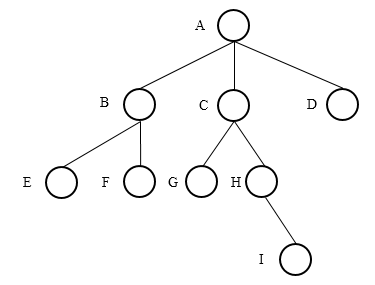
\includegraphics[scale = 0.5]{images/example-tree.png}\\
		\caption{Example Tree}
	\end{figure}

	\textit{\textbf{ Aggregation using binary representation}}
	\[ 
		\begin{array}{lcccc}
			\mbox{Carry} & 0 & 1 & 1 & 0\\
			\hline
			\mbox{Trees in B's forest} & 0 & 0 & 0 & 1 \\
			\mbox{ } & 0 & 0 & 1 & 0 \\
			\hline
			\mbox{Tree in C's forest} & 0 & 1 & 0 & 0 \\
			\hline
			\mbox{Tree in D's forest} & 0 & 0 & 0 & 1 \\
			\hline
			\mbox{A's own message} & 0 & 0 & 0 & 1 \\
			\hline
			\mbox{Aggregation} & 1 & 0 & 0 & 1 
		\end{array}
	\] 

	\subsection{aggregator centric Aggregation-Commit approach}


\newpage
\begin{algorithm}[H]\label{number3} \caption {CommitmentTreeGeneration}
	\begin {algorithmic}[1]

		\STATE depth = \at.MaxDepth
		\WHILE {depth $\geq$ 0}

			\FORALL {\node \   $\in$ \at.depth }

			\STATE \node.\forest = NULL
					\STATE Create (\node.\msg, \sign $_{\cal{N}}$(\node.\msg))
					\STATE Attach (\node.\msg, \sign $_{\cal{N}}$(\node.\msg)) to \node.\forest
					
					\IF {\node.\children \ $\neq$ \ 0}

						\FORALL {\child \ $\in$ \node.\children }

							\FORALL {tree root \treeRoot \ $\in$ \child.\forest}

								\IF {\node \ has \treeRoot.\cert (else get \treeRoot.\cert )} 

									\IF {\node verifies \treeRoot.msg (else raise an alarm)}

										\STATE Add \treeRoot \ to \node.\forest
										
									\ENDIF
								
								\ENDIF

							\ENDFOR

							\STATE \node.\forest \ =	CommitmentTreeCoding ( \node.\forest \ ) 
						
						\ENDFOR
		
					\ENDIF


			\ENDFOR

			\STATE {depth = depth - 1 }

		\ENDWHILE
	\end{algorithmic}
\end{algorithm}

\begin{algorithm}[H]\caption{CommitmentTreeCoding}
	\begin{algorithmic}[1]

		\STATE \temp \ = SortLinkedList( \node.\forest \ )

		\WHILE {\temp.\nextTree \ $\neq$ \ 0}

			\IF {\temp.\height \ $\neq$ \ \temp.\nextTree.\height } 
				\STATE \temp \ = \temp.\nextTree
			\ELSE

				\STATE Create an aggregation node \aggregator 
				\STATE \aggregator.\height \ = \temp.\height \ + 1
				\STATE \aggregator.\lc \ = \temp
				\STATE \aggregator.\rc \ = \temp.\nextTree
				\STATE Insert \aggregator \ to \node.\forest
				\STATE Remove \temp
				\STATE Remove \temp.\nextTree
				\STATE \temp \ = SortLinkedList( \node.\forest \ )

			\ENDIF

		\ENDWHILE		

		\STATE return \temp

	\end{algorithmic}

\end{algorithm}

\newpage

\begin{algorithm}
\caption{Pseudo algorithm to detect a cheater}

	\begin{algorithmic}[1]

			\STATE \querier \ finds out all the \complainer$_{\mathcal{N}}$ $\in$ \at \ using a complainer detecting algorithm

			\FORALL {\complainer$_{\mathcal{N}}$}

				\STATE \querier \ gets \node$_{0}$, \sign $_{\cal{N}}$ ( \node$_{0}$ )
			
			\ENDFOR

			\STATE \querier \  finds possible \cheater \ based on \complainer$_{\mathcal{N}}$

			\FORALL {\cheater}

				\STATE \querier \  gets \node$_{\mathcal{I}}$, \sign $_{\cal{N}}$ ( \node$_{I}$ ) \cheater \  receives and sends. 
				\STATE If needed \querier \  gets \node$_{\mathcal{I}}$, \sign $_{\cal{N}}$ ( \node$_{I}$ ) of the \parent \ \cheater 
			
			\ENDFOR

			\STATE \querier \  determines the \cheater \ based on recived information

	\end{algorithmic}
\end{algorithm}

\textit{Properties of commitment tree and aggregation tree}

	If you have $O(n)$ children then you need atleast $\Omega(n)$ \& at max $O(nlog(n))$ certificates.

	If you have $O(n)$ descendents then you need $\Omega(log(n))$  \& at max $O(nlog(n))$ certificates.


\section{Advantages of this protocol}
\section{Disadvantages of this protocol}
